Prot{\'e}g{\'e}LOV it is an open source tool that provides support to the methodological guidelines described in section \ref{sec:reuse}. It is written in Java programming language as a plugin for the \protege ontology editor. It can be easily installed by just copying the jar file provided at the Prot{\'e}g{\'e}LOV website\footnote{\url{http://lab.isoco.net/prolov/}} into the plugins directory of an existing \protege installation. Then upon a new start, the user should select \emph{Linked Open Vocabularies} item, within the \emph{Ontology views} menu item.

Prot{\'e}g{\'e}LOV provides the following functionalities 

\paragraph{Search for a particular term (class or property) in LOV repository}. %The user selects a particular 

\paragraph{Browse the list of terms, from LOV repository, which matches the search criteria}

\paragraph{Reuse directly a particular term from LOV repository}

\paragraph{Add the particular term and define the rdf:subClassOf/rdfs:subPropertyOf axiom}

\paragraph{Add the particular term and define the owl:equivalentClass/owl:equivalentProperty axiom}


\begin{figure}[!bht]
\center
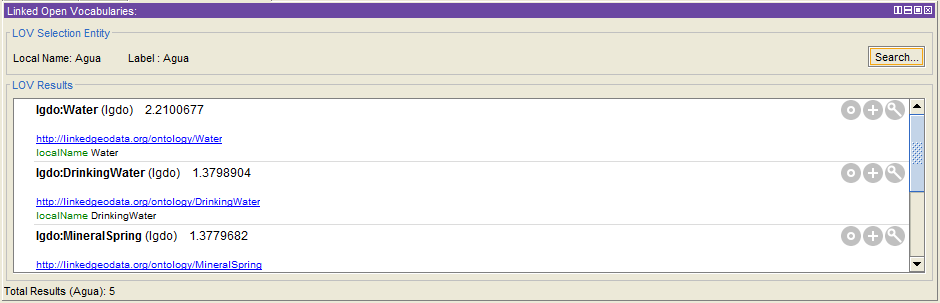
\includegraphics[scale=0.5]{img/LOVmockup.png}
\label{fig:LOVresults}
\caption{Panel showing the results for searching a term in the class hierarchy.}
\end{figure}


\begin{figure}[!bht]
\center
\includegraphics[scale=0.5]{img/LOVOptions.png}
\caption{Three actions currently available in the plugin after looking up a term in LOV catalogue: (a) reuse direct, (b) add equivalent axiom and (c) add subClass axiom}
\label{fig:LOVoptions}
\end{figure}
